\documentclass[aspectratio=169, 10pt]{beamer}

\usetheme{Madrid}

\usepackage{amsmath, amssymb}
\usepackage{bm}
\usepackage{tikz}
\usetikzlibrary{positioning, arrows.meta}
\usepackage{booktabs}
\usepackage{mathtools}

\definecolor{mblue}{RGB}{0,70,140}
\setbeamercolor{structure}{fg=mblue}
\setbeamercolor{palette primary}{bg=mblue, fg=white}
\setbeamercolor{palette secondary}{bg=mblue!80, fg=white}
\setbeamercolor{palette tertiary}{bg=mblue!60, fg=white}
\setbeamercolor{palette quaternary}{bg=mblue!40, fg=black}

\setbeamertemplate{blocks}[rounded][shadow=false]

\setbeamercolor{block title}{bg=mblue, fg=white}
\setbeamercolor{block body}{bg=mblue!10, fg=black}
\setbeamercolor{block title alerted}{bg=red!70!black, fg=white}
\setbeamercolor{block body alerted}{bg=red!10, fg=black}
\setbeamercolor{block title example}{bg=green!45!black, fg=white}
\setbeamercolor{block body example}{bg=green!10, fg=black}

\title[Rosetta Stone Problem]{The Incomplete Rosetta Stone Problem}
\subtitle{Identifiability Results for Multi-View Nonlinear ICA}
\author[Gresele et al.\ 2020]{%
  L.~Gresele \and P.K.~Rubenstein \and A.~Mehrjou \and
  F.~Locatello \and B.~Schölkopf}
\institute[UAI 2020]{Uncertainty in Artificial Intelligence (UAI), 2020}
\date{Presented by Nicola Debole}

\tikzset{
  latent/.style  = {circle, draw, thick, minimum size=0.85cm, font=\small},
  observed/.style= {circle, draw, thick, fill=gray!25, minimum size=0.85cm, font=\small},
  arr/.style     = {->, >=Stealth, thick}
}

% ---------------------------------------------------------------
\begin{document}
% ---------------------------------------------------------------

\maketitle

% ============================================================
% SLIDE 1: HISTORY (1/2)
% ============================================================
\begin{frame}{A Brief History of ICA Identifiability (1/2)}
  \textbf{Independent Component Analysis (ICA):} recover $\mathbf{s}$ from a single observation
  $\mathbf{x}=\mathbf{f}(\mathbf{s})$

  \bigskip
  \begin{block}{Linear ICA: Identifiable \hfill\normalfont\small Darmois 1953; Comon 1994}
    If $\mathbf{f}$ is linear, the model is identifiable up to permutation and scaling of
    sources; provided at most one component is Gaussian.
  \end{block}

  \bigskip
  \begin{alertblock}{Nonlinear ICA: Provably Non-Identifiable
      \hfill\normalfont\small Hyvärinen \& Pajunen, 1999}
    For an arbitrary nonlinear $\mathbf{f}$:
    \begin{itemize}
      \item Infinitely many $(\mathbf{f}',\mathbf{s}')$ pairs are consistent with the same
            observed data distribution $p(\mathbf{x})$
      \item For any smooth bijection $\varphi$, the pair
            $\bigl(\mathbf{f}\circ\varphi^{-1},\;\varphi(\mathbf{s})\bigr)$
            produces the identical $p(\mathbf{x})$ (equally valid, but different sources)
    \end{itemize}
    \[
      \Rightarrow \text{Without further constraints, } \mathbf{s}
      \textbf{ cannot be recovered}
    \]
  \end{alertblock}
\end{frame}

% ============================================================
% SLIDE 2: HISTORY (2/2)
% ============================================================
\begin{frame}{A Brief History of ICA Identifiability (2/2): Auxiliary Variables}
  \textbf{Breakthrough:} condition independence on an auxiliary variable $\mathbf{u}$
  \hfill{\small Hyvärinen, Sasaki \& Turner, 2019}

  \bigskip
  \begin{block}{Conditional Independence Model}
    Replace unconditional independence of $\mathbf{s}$ with:
    \[
      \log p(\mathbf{s}\mid\mathbf{u}) = \sum_i q_i(s_i,\,\mathbf{u})
    \]
    Under this and a \emph{variability} condition on $\mathbf{u}$, the model
    \textbf{becomes identifiable}.
  \end{block}

  \bigskip
  \textbf{Key limitation:} requires observing the auxiliary variable $\mathbf{u}$
  \begin{itemize}
    \item $\mathbf{u}$ may be unknown, hidden, or costly to observe
    \item E.g.\ in an audio recording, $\mathbf{u}$ = the previous time segment:
          adjacent frames share the same acoustic context, but this requires
          access to the temporal ordering of the data
  \end{itemize}

\end{frame}

% ============================================================
% SLIDE 3: SETTING
% ============================================================
\begin{frame}{Setting: The Generative Model}
  \begin{columns}[T]
    \column{0.60\textwidth}
      \textbf{Two views of a shared latent source $\mathbf{s}$:}
      \begin{align*}
        \mathbf{x}_1 &= \mathbf{f}_1(\mathbf{s})\\
        \mathbf{x}_2 &= \mathbf{f}_2(\mathbf{s})\\
        p(\mathbf{s}) &= \prod_i p_i(s_i)
      \end{align*}
      \begin{itemize}
        \item $\mathbf{s}=(s_1,\ldots,s_D)\in\mathbb{R}^D$: \textbf{mutually independent} components
        \item $\mathbf{f}_1,\mathbf{f}_2$: smooth, invertible, \emph{unknown} nonlinear mixings
        \item $\mathbf{x}_1,\mathbf{x}_2$ observed; $\mathbf{s}$ latent
        \item \textbf{Goal:} recover $\mathbf{s}$ from $(\mathbf{x}_1,\mathbf{x}_2)$ only
      \end{itemize}
      \medskip
      % ,\textbf{Rosetta Stone metaphor:}\\
      % two texts in different unknown languages sharing a
      % common underlying meaning: the shared $\mathbf{s}$ is the key

    \column{0.36\textwidth}
      \centering\vspace{1em}
      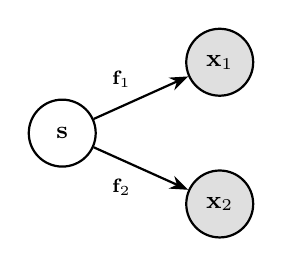
\begin{tikzpicture}
        \node[latent]   (s)  at (0,0)    {$\mathbf{s}$};
        \node[observed] (x1) at (2, 0.9) {$\mathbf{x}_1$};
        \node[observed] (x2) at (2,-0.9) {$\mathbf{x}_2$};
        \draw[arr] (s) -- node[above left, font=\scriptsize]{$\mathbf{f}_1$} (x1);
        \draw[arr] (s) -- node[below left, font=\scriptsize]{$\mathbf{f}_2$} (x2);
      \end{tikzpicture}\\[0.6em]
      \small Shaded = observed
  \end{columns}
\end{frame}

% ============================================================
% SLIDE 4: MULTI-VIEW SETTING
% ============================================================
\begin{frame}{Non-Linear ICA with Multiple Views}
  \textbf{Key idea:} jointly observing $(\mathbf{x}_1,\mathbf{x}_2)$ constrains the inverse problem enough for
  identifiability

  \bigskip
  \begin{center}
    \textbf{Contrastive learning task:} train a classifier to distinguish
  \end{center}
  \begin{columns}
    \column{0.44\textwidth}\centering
      \textcolor{green!55!black}{\textbf{Positive pairs}}\\
      $(\mathbf{x}_1,\mathbf{x}_2)$: \emph{same} realisation of $\mathbf{s}$
    \column{0.08\textwidth}\centering vs.
    \column{0.44\textwidth}\centering
      \textcolor{red!70!black}{\textbf{Negative pairs}}\\
      $(\mathbf{x}_1,\mathbf{x}_2^*)$: \emph{different} realisations of $\mathbf{s}$
  \end{columns}

  \bigskip
  \textbf{Requirements:}
  \begin{itemize}
    \item \textbf{Component-wise corruption:}
      \[
        \mathbf{x}_i = \mathbf{f}_i\!\bigl(\mathbf{g}_i(\mathbf{s},\mathbf{n}_i)\bigr),
        \quad
        \mathbf{n}_i \perp\!\!\!\perp \mathbf{s},
        \quad
        g_{ij}(\mathbf{s},\mathbf{n}_i) = g_{ij}(s_j, n_{ij})
      \]
      Noise acts on each source dimension \emph{independently}, before mixing by $\mathbf{f}_i$
    \item $\mathbf{f}_i$ invertible; at least one view must be stochastic (some noise)
    \item \textbf{Sufficiently Distinct Views (SDV)}, discussed in the limitations section
  \end{itemize}
\end{frame}

% ============================================================
% SLIDE 5: LOG MI: GAN DISCRIMINATOR
% ============================================================
\begin{frame}{Log MI: Optimal GAN Discriminator}
  \textbf{Setup:} train a classifier $C\colon(\mathbf{x}_1,\mathbf{x}_2)\to[0,1]$ to distinguish positive from
  negative pairs with equal class probabilities:
  \[
    \underbrace{p(\mathbf{x}_1,\mathbf{x}_2)}_{\text{positive (class 0)}}
    \quad\text{vs.}\quad
    \underbrace{p(\mathbf{x}_1)\,p(\mathbf{x}_2)}_{\text{negative (class 1)}}
  \]

  \bigskip
  \begin{theorem}[Optimal discriminator (Goodfellow et al., 2014)]
    The optimal binary classifier for a symmetric binary classification task satisfies:
    \[
      C^*(\mathbf{x}) = \frac{P_0(\mathbf{x})}{P_0(\mathbf{x}) + P_1(\mathbf{x})}
    \]
  \end{theorem}

  \medskip
  In our setting ($P_0 = p(\mathbf{x}_1,\mathbf{x}_2)$, $P_1 = p(\mathbf{x}_1)p(\mathbf{x}_2)$):
  \[
    C^*(\mathbf{x}_1,\mathbf{x}_2)
    = \frac{p(\mathbf{x}_1,\mathbf{x}_2)}{p(\mathbf{x}_1,\mathbf{x}_2)+p(\mathbf{x}_1)p(\mathbf{x}_2)}
    = \sigma\!\left(\log\frac{p(\mathbf{x}_1,\mathbf{x}_2)}{p(\mathbf{x}_1)p(\mathbf{x}_2)}\right)
  \]

\end{frame}

% ============================================================
% SLIDE 6: BRIDGE: WHY LOG MI?
% ============================================================
\begin{frame}{Why Log Mutual Information?}
  We have a binary classification task: distinguish
  \[
    \underbrace{p(\mathbf{x}_1,\mathbf{x}_2)}_{\text{positive (shared }\mathbf{s}\text{)}}
    \quad\text{vs.}\quad
    \underbrace{p(\mathbf{x}_1)\,p(\mathbf{x}_2)}_{\text{negative (independent)}}
  \]

  \bigskip
  \textbf{Key question:} what does the \emph{optimal} classifier actually compute?

  \bigskip
  \begin{block}{The bridge (Goodfellow et al., 2014)}
    The optimal Bayes classifier for this symmetric task outputs a monotone function of
    the \textbf{pointwise log mutual information}:
    \[
      \log \frac{p(\mathbf{x}_1,\mathbf{x}_2)}{p(\mathbf{x}_1)\,p(\mathbf{x}_2)}
    \]
  \end{block}

  \bigskip
  \begin{itemize}
    \item Training the classifier $\equiv$ learning the log MI
    \item The structure of the log MI directly encodes the sources $\mathbf{s}$
    \item All identifiability results in the paper exploit this structure
  \end{itemize}
\end{frame}

%% ============================================================
%% SLIDE 7: LOG MI: DEFINITION (commented out, may be useful later)
%% ============================================================
%\begin{frame}{Log Mutual Information: Definition}
%  \textbf{Pointwise log mutual information:}
%  \[
%    \log\frac{p(\mathbf{x}_1,\mathbf{x}_2)}{p(\mathbf{x}_1)\,p(\mathbf{x}_2)}
%    \;=\;
%    \log p(\mathbf{x}_1,\mathbf{x}_2)
%    \;-\;
%    \log p(\mathbf{x}_1)
%    \;-\;
%    \log p(\mathbf{x}_2)
%  \]
%
%  \bigskip
%  \begin{columns}
%    \column{0.48\textwidth}
%    \begin{block}{Independent case: $\mathbf{x}_1\perp\!\!\!\perp\mathbf{x}_2$ (no shared $\mathbf{s}$)}
%      \[
%        p(\mathbf{x}_1,\mathbf{x}_2) = p(\mathbf{x}_1)\,p(\mathbf{x}_2)
%      \]
%      \[
%        \text{ratio}=1 \;\Rightarrow\; \log\text{MI}=0
%      \]
%    \end{block}
%
%    \column{0.48\textwidth}
%    \begin{block}{Dependent case: shared $\mathbf{s}$}
%      \[
%        p(\mathbf{x}_1,\mathbf{x}_2) \neq p(\mathbf{x}_1)\,p(\mathbf{x}_2)
%      \]
%      \[
%        \log\text{MI} \neq 0
%      \]
%      Positive / negative depending on the correlation direction
%    \end{block}
%  \end{columns}
%
%  \bigskip
%  \textbf{Intuition:} the log MI measures how much more likely a pair $(\mathbf{x}_1,\mathbf{x}_2)$ is under the joint distribution compared to if the two views were independent
%\end{frame}

%% ============================================================
%% SLIDE 8: LOG MI: KEY FACTORISATION (commented out, may be useful later)
%% ============================================================
%\begin{frame}{Log MI: The Key Factorisation}
%  Under the component-wise corruption model, the log MI decomposes \textbf{component-wise}:
%
%  \bigskip
%  \[
%    \log p(\mathbf{x}_1,\mathbf{x}_2) - \log p(\mathbf{x}_1)\,p(\mathbf{x}_2)
%    \;=\;
%    \sum_i \alpha_i\!\bigl(s_i,\,g_i(s_i,n_i)\bigr)
%    \;-\;
%    \sum_i \delta_i\!\bigl(g_i(s_i,n_i)\bigr)
%  \]
%  where $s_i = f_{1,i}^{-1}(\mathbf{x}_1)$ and $g_i(s_i,n_i) = f_{2,i}^{-1}(\mathbf{x}_2)$.
%
%  \bigskip
%  \textbf{Why this is the central structural result:}
%  \begin{itemize}
%    \item Each term depends on only \textbf{one component} of $\mathbf{s}$ at a time
%    \item The log MI is a sum of per-component contributions (no cross-component terms)
%    \item A classifier trained to estimate the log MI \textbf{must} learn this component-wise structure
%    \item $\Rightarrow$ the classifier's internal representation encodes the \textbf{independent components of $\mathbf{s}$}
%  \end{itemize}
%
%  \medskip
%  This factorisation is the engine behind \emph{all} identifiability proofs in the paper.
%\end{frame}

%% ============================================================
%% SLIDE 9: LOG MI: COUNTERFACTUAL + SHUFFLING (commented out, may be useful later)
%% ============================================================
%\begin{frame}{Log MI: Counterfactual Interpretation \& Shuffling Trick}
%  \begin{columns}[T]
%    \column{0.50\textwidth}
%      \textbf{What is $p(\mathbf{x}_1)\,p(\mathbf{x}_2)$?}
%
%      \bigskip
%      \begin{block}{Counterfactual Distribution}
%        $p(\mathbf{x}_1)\,p(\mathbf{x}_2)$ is the distribution of $(\mathbf{x}_1,\mathbf{x}_2)$ \emph{if
%        the two views shared no common source}
%
%        \medskip
%        \textit{``What would $\mathbf{x}_2$ look like if it came from a \textbf{different} $\mathbf{s}$ than $\mathbf{x}_1$?''}
%
%        \medskip
%        $\to$ removes \emph{all} information shared between views
%      \end{block}
%
%    \column{0.46\textwidth}
%      \textbf{Sampling via batch shuffling}
%
%      \medskip
%      We never compute $p(\mathbf{x}_1)\,p(\mathbf{x}_2)$ analytically.
%      Instead:
%      \begin{enumerate}
%        \item Draw $\mathbf{x}_1^{(i)}$ from sample $i$;
%              draw $\mathbf{x}_2^{(j)}$ from sample $j\neq i$
%        \item Different index $\Rightarrow$ different $\mathbf{s}$ $\Rightarrow$
%              pair is from $p(\mathbf{x}_1)\,p(\mathbf{x}_2)$
%      \end{enumerate}
%
%      \medskip
%      These are the \textbf{negative pairs} in contrastive learning.
%
%      \medskip
%      No density estimation required:
%      just re-pair samples within the batch!
%  \end{columns}
%\end{frame}

% ============================================================
% SLIDE 10: ONE NOISELESS VIEW: SETTING
% ============================================================
\begin{frame}{One Noiseless View: Setting}
  \begin{columns}[T]
    \column{0.56\textwidth}
      \textbf{Generative model (§3.1):}
      \begin{align*}
        \mathbf{x}_1 &= \mathbf{f}_1(\mathbf{s}) & &\text{(noiseless)}\\
        \mathbf{x}_2 &= \mathbf{f}_2\!\bigl(\mathbf{g}(\mathbf{s},\mathbf{n})\bigr) & &\text{(noisy)}
      \end{align*}
      \[
        p(\mathbf{s})=\prod_i p_i(s_i),\quad
        p(\mathbf{n})=\prod_i p_i(n_i),\quad
        \mathbf{n}\perp\!\!\!\perp\mathbf{s}
      \]

      \bigskip
      \begin{itemize}
        \item $\mathbf{g}$ is \textbf{component-wise}: corrupts each $s_i$ independently
        \item $\mathbf{f}_1,\mathbf{f}_2$: arbitrary nonlinear invertible mixings
      \end{itemize}

      \bigskip
      \textbf{Practical motivation:}\\
      one precise instrument + one noisy device\\
      (e.g.\ high-quality fMRI + fast-but-noisy EEG)

    \column{0.40\textwidth}
      \centering\vspace{1em}
      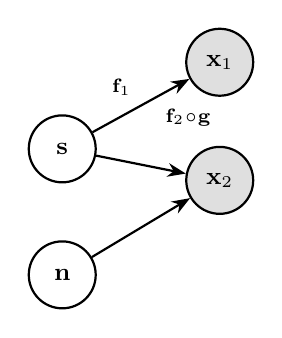
\begin{tikzpicture}
        \node[latent]   (s)  at (0, 0)   {$\mathbf{s}$};
        \node[observed] (x1) at (2, 1.1) {$\mathbf{x}_1$};
        \node[latent]   (n)  at (0,-1.6) {$\mathbf{n}$};
        \node[observed] (x2) at (2,-0.4) {$\mathbf{x}_2$};
        \draw[arr] (s)  -- node[above left, font=\scriptsize]{$\mathbf{f}_1$} (x1);
        \draw[arr] (s)  -- (x2);
        \draw[arr] (n)  -- (x2);
        \node[font=\scriptsize] at (1.6, 0.4) {$\mathbf{f}_2\!\circ\!\mathbf{g}$};
      \end{tikzpicture}\\[0.5em]
      \small Shaded = observed
  \end{columns}
\end{frame}

% ============================================================
% SLIDE 10: ONE NOISELESS VIEW: THEOREM 1
% ============================================================
\begin{frame}{One Noiseless View: Theorem 1}
  \begin{theorem}[Theorem 1 (informal)]
    Suppose $\boldsymbol{\alpha}$ satisfies the SDV assumption. Train a classifier using the
    regression function:
    \[
      r(\mathbf{x}_1,\mathbf{x}_2) = \sum_i \psi_i\!\bigl(h_i(\mathbf{x}_1),\;\mathbf{x}_2\bigr)
    \]
    where $\mathbf{h}=(h_1,\ldots,h_D)$ are invertible smooth functions with smooth inverses.

    \medskip
    Then in the infinite-data, infinite-capacity limit, $\mathbf{h}$ \textbf{inverts $\mathbf{f}_1$} up to
    component-wise invertible transformations: the $h_i(\mathbf{x}_1)$ recover the independent
    components of $\mathbf{s}$.
  \end{theorem}

  \bigskip
  \textbf{What this gives us:}
  \begin{itemize}
    \item Exact recovery of $\mathbf{s}$ from the noiseless view $\mathbf{x}_1$ (up to per-component scalar)
    \item The factorised form of $r$ forces each $\psi_i$ to depend on a single source component
  \end{itemize}

  \medskip
  \textbf{Proof sketch:} component-wise factorisation of log MI $\;\Rightarrow\;$ each $\psi_i$ term must
  match the corresponding $\alpha_i$ term $\;\Rightarrow\;$ $h_i$ must invert $f_{1,i}$
\end{frame}

% ============================================================
% SLIDE 11: ONE NOISELESS VIEW: COROLLARY 3 + THEOREM 4
% ============================================================
\begin{frame}{One Noiseless View: Corollary 3 \& Theorem 4}
  \begin{block}{Corollary 3: Recovering from the \emph{noisy} view}
    Using an alternative factorisation of the log MI with
    $r(\mathbf{x}_1,\mathbf{x}_2)=\sum_i \psi_i(\mathbf{x}_1, h_i(\mathbf{x}_2))$,\\
    $\mathbf{h}$ inverts $\mathbf{f}_2$ in the sense that $h_i(\mathbf{x}_2)$ recovers
    $g_i(s_i,n_i)$ up to component-wise invertible transformations.
  \end{block}

  \bigskip
  \begin{theorem}[Theorem 4: Aligned joint recovery]
    If \emph{both} $\boldsymbol{\alpha}$ and $\boldsymbol{\gamma}$ satisfy SDV, using:
    \[
      r(\mathbf{x}_1,\mathbf{x}_2) = \sum_i \psi_i\!\bigl(h_{1,i}(\mathbf{x}_1),\;h_{2,i}(\mathbf{x}_2)\bigr)
    \]
    $\mathbf{h}_1$ and $\mathbf{h}_2$ invert $\mathbf{f}_1$ and $\mathbf{f}_2$ respectively, and are \textbf{aligned}:
    \[
      h_{1,i}(\mathbf{x}_1) \;\perp\!\!\!\perp\; h_{2,j}(\mathbf{x}_2)
      \quad \forall\, i\neq j
    \]
  \end{theorem}

  \medskip
  \textbf{Alignment matters:} component $i$ from view 1 corresponds to component $i$ from view 2;
  both representations refer to the \emph{same} source factor
\end{frame}

% ============================================================
% SLIDE 12: TWO NOISY VIEWS
% ============================================================
\begin{frame}{Two Noisy Views}
  \begin{columns}[T]
    \column{0.56\textwidth}
      \textbf{Setting (§3.2):}
      \[
        \mathbf{x}_i = \mathbf{f}_i\!\bigl(\mathbf{g}_i(\mathbf{s},\mathbf{n}_i)\bigr),\quad i=1,2
      \]
      Both views corrupted; exact recovery of $\mathbf{s}$ is impossible.

      \bigskip
      \begin{theorem}[Theorem 5 (informal)]
        If $\boldsymbol{\eta}$ and $\boldsymbol{\lambda}$ satisfy SDV, the algorithm recovers
        $\mathbf{g}_1(\mathbf{s},\mathbf{n}_1)$ and $\mathbf{g}_2(\mathbf{s},\mathbf{n}_2)$
        with \textbf{aligned} representations.
      \end{theorem}

      \begin{itemize}
        \item As noise $\to 0$:\;
              $\mathbf{g}_i(\mathbf{s},\mathbf{n}_i)\to\mathbf{s}$\;
              $\Rightarrow$ exact recovery (Corollary 6)
        \item Practical setting: two different modalities at different noise levels
          (e.g.\ simultaneous fMRI + optical imaging)
      \end{itemize}

    \column{0.40\textwidth}
      \centering\vspace{0.8em}
      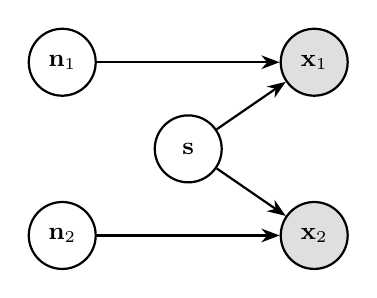
\begin{tikzpicture}
        \node[latent]   (s)  at (0, 0)    {$\mathbf{s}$};
        \node[latent]   (n1) at (-1.6, 1.1) {$\mathbf{n}_1$};
        \node[latent]   (n2) at (-1.6,-1.1) {$\mathbf{n}_2$};
        \node[observed] (x1) at ( 1.6, 1.1) {$\mathbf{x}_1$};
        \node[observed] (x2) at ( 1.6,-1.1) {$\mathbf{x}_2$};
        \draw[arr] (s)  -- (x1);
        \draw[arr] (n1) -- (x1);
        \draw[arr] (s)  -- (x2);
        \draw[arr] (n2) -- (x2);
      \end{tikzpicture}
  \end{columns}
\end{frame}

% ============================================================
% SLIDE 13: MULTIPLE NOISY VIEWS
% ============================================================
\begin{frame}{Multiple Noisy Views}
  \textbf{Setting (§3.3):} $N$ simultaneous noisy views of $\mathbf{s}$
  \[
    \mathbf{x}_i = \mathbf{f}_i\!\bigl(\mathbf{g}_i(\mathbf{s},\mathbf{n}_i)\bigr),
    \quad i=1,\ldots,N
  \]

  \medskip
  \textbf{Central question:} as $N\to\infty$, can we recover $\mathbf{s}$ \emph{exactly}
  even when every view is noisy?

  \bigskip
  \begin{theorem}[Theorem 8 (informal)]
    If the per-view noises $\mathbf{n}_i$ are mutually independent across views and the
    corruption functions $\mathbf{g}_i$ (parameterised by $\boldsymbol{\lambda}_i$) satisfy
    the SDV condition with bounded noise variance, then exact recovery of $\mathbf{s}$ up
    to affine ambiguity is possible in the limit $N\to\infty$.
  \end{theorem}

  \bigskip
  \textbf{Intuition:} the proof applies the \textbf{Kolmogorov Strong Law of Large Numbers}:
  given independent random variables with bounded variances, their running average converges
  \emph{almost surely} to the true mean.
  Since the noises $\mathbf{n}_i$ are independent and zero-mean, the per-view corruptions
  cancel out in the average, leaving only $\mathbf{s}$:
  \[
    \mathbf{s}
    \;\approx\;
    \Omega^N(\mathbf{s},\mathbf{n})
    = \frac{1}{N}\sum_{i=1}^N e_i\circ k_i(\mathbf{s}+\mathbf{n}_i)
    \;\xrightarrow{N\to\infty}\;\mathbf{s}
    \quad\text{(a.s.)}
  \]
\end{frame}

% ============================================================
% SLIDE 14: LIMITATIONS: SDV
% ============================================================
\begin{frame}{Limitations: Sufficiently Distinct Views (SDV)}
  \begin{definition}[Sufficiently Distinct Views (Definition 2)]
    Functions $\alpha_i(y_i,t_i)$ satisfy SDV if for any $\mathbf{y}$,
    there exist $2D$ distinct values $\mathbf{t}_j$, $j=1,\ldots,2D$, such that the vectors
    \[
      \mathbf{w}_{\boldsymbol{\alpha}}(\mathbf{y},\mathbf{t}_j)
      =\bigl(\alpha_1'',\ldots,\alpha_D'',\,\alpha_1',\ldots,\alpha_D'\bigr)
    \]
    are \textbf{linearly independent}
    \hfill
    $\bigl(\alpha_i'=\partial\alpha_i/\partial t,\;\alpha_i''=\partial^2\alpha_i/\partial t^2\bigr)$
  \end{definition}

  \begin{alertblock}{Note}
    The derivation of this definition may be incorrect; treat with caution.
  \end{alertblock}

  \medskip
  \textbf{Informal meaning:} the conditional log-probability of the corruption must vary
  \emph{sufficiently} as a function of the source value

  \medskip
  \begin{itemize}
    \item Connected to the ``Variability'' assumption of Hyvärinen et al.\ [2019]
    \item \textbf{Violated} if the two views are identical $\Rightarrow$ no new information
          $\Rightarrow$ no identifiability
    \item The noise variables $\mathbf{n}_i$ are \textbf{essential}: SDV cannot hold in a
          fully deterministic setting
  \end{itemize}

\end{frame}

% ============================================================
% SLIDE 15: LIMITATIONS: COMPONENT-WISE CORRUPTER
% ============================================================
\begin{frame}{Limitations: Component-wise Corrupter in Practice}
  \textbf{Theory requires:} $\mathbf{g}$ corrupts $\mathbf{s}$ \emph{component-wise}:
  noise acts on each latent factor \emph{before} mixing by $\mathbf{f}$

  \bigskip
  \begin{alertblock}{Problem: Standard Augmentations Act on $\mathbf{x}$, Not on $\mathbf{s}$}
    Cropping, colour jitter, Gaussian blur, etc.\ transform \textbf{pixels}\\
    $\Rightarrow$ corruption is applied to $\mathbf{x}$, not component-wise to $\mathbf{s}$
    $\Rightarrow$ model assumptions are violated
  \end{alertblock}

  \bigskip
  \textbf{Example: Shapes3D dataset}
  \begin{itemize}
    \item Has explicit generative factors: floor colour, wall colour, object shape, scale,
          orientation, \ldots
    \item Looks ideal on paper, but \textbf{no mechanism to inject noise at the factor level}
          before rendering
    \item Any augmentation applied post-rendering operates on $\mathbf{x}$, not on $\mathbf{s}$
    \item $\Rightarrow$ the component-wise corruption assumption is violated
  \end{itemize}

  \bigskip
  \textbf{Conclusion:} it is \textbf{hard to find a dataset that genuinely satisfies the model}:
  the data generation pipeline must expose a separable noise injection point at the level of
  the generative factors $\mathbf{s}$
\end{frame}

% ---------------------------------------------------------------
\appendix
% ---------------------------------------------------------------

% ============================================================
% APPENDIX TITLE
% ============================================================
\begin{frame}[plain]
  \centering\vfill
  {\Large\textbf{Appendix: Proof Sketches}}\\[1em]
  \normalsize
  Theorems 1, 4, 5, 8 \quad Corollaries 3, 6 \quad Lemma 7
  \vfill
\end{frame}

% ============================================================
% APPENDIX A — SDV DEFINITION: EQS. 9-11 AND DERIVATIVE DIRECTION
% ============================================================
\begin{frame}{SDV: Formal Definition and Proof-Correctness Subtlety}
  \begin{definition}[Definition 2 --- Sufficiently Distinct Views]
    Let $\alpha_i(y_i, t_i)$, $i=1,\ldots,N$ be functions of two arguments.
    Denote by $\boldsymbol{\alpha}$ the vector of functions and define
    \begin{align}
      \alpha_i'(y_i,\,t_i) &= \partial\alpha_i(y_i,t_i)/\partial t, \tag{9}\\
      \alpha_i''(y_i,\,t_i) &= \partial^2\alpha_i(y_i,t_i)/\partial t^2, \tag{10}\\
      \mathbf{w}_{\boldsymbol{\alpha}}(\mathbf{y},\mathbf{t})
        &= \bigl(\alpha_1'',\ldots,\alpha_D'',\;\alpha_1',\ldots,\alpha_D'\bigr). \tag{11}
    \end{align}
    $\boldsymbol{\alpha}$ satisfies SDV if for any $\mathbf{y}$, $\exists\; 2D$ distinct values
    $\mathbf{t}_j$ such that $\{\mathbf{w}_{\boldsymbol{\alpha}}(\mathbf{y},\mathbf{t}_j)\}_{j=1}^{2D}$
    are linearly independent.
  \end{definition}

  \begin{alertblock}{Proof of Theorem 1 requires derivatives w.r.t.\ the first argument}
    The proof differentiates $r^*(\mathbf{x}_1,\mathbf{x}_2)=\log\mathrm{MI}$
    w.r.t.\ $\mathbf{x}_1$, which encodes $y_i = s_i$ (the \emph{first} argument of
    $\alpha_i$). The linear system that SDV must render non-singular involves
    $\partial\alpha_i/\partial y_i$ and $\partial^2\alpha_i/\partial y_i^2$, not the
    $t$-derivatives in Eqs.\ (9)--(10).

    \smallskip
    $\Rightarrow$ For correctness, Eqs.\ (9)--(10) should use $\partial/\partial y$
    (first argument); $\partial/\partial t$ is appropriate for Corollary~3, which
    recovers $\mathbf{x}_2$.
  \end{alertblock}
\end{frame}

% ============================================================
% APPENDIX B — KEY FACTORISATION DERIVATION
% ============================================================
\begin{frame}{Proof: Key Log-MI Factorisation (Equation 8)}
  \textbf{Goal:} show $\log p(\mathbf{x}_1,\mathbf{x}_2)-\log p(\mathbf{x}_1)p(\mathbf{x}_2)$
  decomposes component-wise.

  \medskip
  Since $\mathbf{x}_1=\mathbf{f}_1(\mathbf{s})$ is invertible:
  \[
    \log p(\mathbf{x}_2\mid\mathbf{x}_1) - \log p(\mathbf{x}_2)
    = \log p(\mathbf{x}_2\mid\mathbf{s}) - \log p(\mathbf{x}_2)
  \]

  Since $\mathbf{x}_2 = \mathbf{f}_2(\mathbf{g}(\mathbf{s},\mathbf{n}))$ with
  $\mathbf{g}$ \emph{component-wise} and $\mathbf{n}\perp\!\!\!\perp\mathbf{s}$:
  \[
    \log p(\mathbf{x}_2\mid\mathbf{s}) - \log p(\mathbf{x}_2)
    = \sum_i \bigl[\log p(g_i(s_i,n_i)\mid s_i) - \log p(g_i(s_i,n_i))\bigr]
    + \log\det J
  \]

  The Jacobians introduced by $\mathbf{f}_2^{-1}$ cancel between the two terms, giving:
  \[
    \boxed{
      \log p(\mathbf{x}_1,\mathbf{x}_2) - \log p(\mathbf{x}_1)p(\mathbf{x}_2)
      = \sum_i \alpha_i(s_i, g_i(s_i,n_i)) - \sum_i \delta_i(g_i(s_i,n_i))
    }
  \]

  \textbf{Key point:} each term depends on only \emph{one} index $i$ — no cross-component coupling.
\end{frame}

% ============================================================
% APPENDIX C — THEOREM 1 PROOF SKETCH
% ============================================================
\begin{frame}{Proof Sketch: Theorem 1 (One Noiseless View)}
  \textbf{Setting:} $\mathbf{x}_1=\mathbf{f}_1(\mathbf{s})$,
  $\mathbf{x}_2=\mathbf{f}_2(\mathbf{g}(\mathbf{s},\mathbf{n}))$,
  classifier $r(\mathbf{x}_1,\mathbf{x}_2)=\sum_i\psi_i(h_i(\mathbf{x}_1),\mathbf{x}_2)$.

  \medskip
  \begin{enumerate}
    \item \textbf{Factorisation:} the log MI equals
          $\sum_i\alpha_i(s_i,g_i(s_i,n_i))-\sum_i\delta_i(g_i(s_i,n_i))$
          (Appendix A above).
    \item \textbf{Infinite-data optimum:} in the limit of infinite data and universal
          approximation, $r^*$ must equal the log MI everywhere.
    \item \textbf{Functional matching:} $r$ depends on $\mathbf{x}_1$ only through
          $h_i(\mathbf{x}_1)$. The log MI depends on $\mathbf{x}_1$ only through
          $s_i = f_{1,i}^{-1}(\mathbf{x}_1)$. Hence $h_i(\mathbf{x}_1)$ must be a
          function of $s_i$ alone.
    \item \textbf{SDV (uniqueness):} the SDV condition on $\boldsymbol{\alpha}$ ensures
          the mapping from $h_i(\mathbf{x}_1)$ to $s_i$ is invertible. Without SDV,
          multiple $h_i$'s could achieve the same loss.
  \end{enumerate}

  \medskip
  \textbf{Conclusion:} $h_i(\mathbf{x}_1)$ recovers $s_i$ up to a component-wise
  invertible transformation. Full proof: Appendix D.1 of the paper.
\end{frame}

% ============================================================
% APPENDIX C — COROLLARY 3 PROOF SKETCH
% ============================================================
\begin{frame}{Proof Sketch: Corollary 3 (Recovering from the Noisy View)}
  \textbf{Alternative factorisation} (Equation 12):
  \[
    \log p(\mathbf{x}_1,\mathbf{x}_2) - \log p(\mathbf{x}_1)p(\mathbf{x}_2)
    = \sum_i \gamma_i(s_i,g_i(s_i,n_i)) - \sum_i \beta_i(s_i)
  \]
  Now the \emph{second} argument carries the $\mathbf{x}_2$ dependence.

  \medskip
  \textbf{Key change:} use regression function
  $r(\mathbf{x}_1,\mathbf{x}_2) = \sum_i\psi_i(\mathbf{x}_1, h_i(\mathbf{x}_2))$.

  \medskip
  Repeating the Theorem 1 argument:
  \begin{enumerate}
    \item $r^*$ must equal the log MI in the infinite-data limit.
    \item The log MI now depends on $\mathbf{x}_2$ only through $g_i(s_i,n_i)$.
    \item Therefore $h_i(\mathbf{x}_2)$ recovers $g_i(s_i,n_i)$ up to component-wise
          invertible transformations.
    \item SDV on $\boldsymbol{\gamma}$ ensures uniqueness.
  \end{enumerate}

  \medskip
  \textbf{Note:} this gives access to the \emph{corrupted} source $g_i(s_i,n_i)$, not to
  $s_i$ directly — the noise $n_i$ cannot be disentangled from $s_i$ using this view alone.
\end{frame}

% ============================================================
% APPENDIX D — THEOREM 4 PROOF SKETCH
% ============================================================
\begin{frame}{Proof Sketch: Theorem 4 (Aligned Joint Recovery)}
  \textbf{Setting:} both $\boldsymbol{\alpha}$ and $\boldsymbol{\gamma}$ satisfy SDV.
  Use $r(\mathbf{x}_1,\mathbf{x}_2)=\sum_i\psi_i(h_{1,i}(\mathbf{x}_1),h_{2,i}(\mathbf{x}_2))$.

  \medskip
  \begin{enumerate}
    \item \textbf{Component-wise recovery (from Thm 1 \& Cor 3):}
          SDV on $\boldsymbol{\alpha}$ forces $h_{1,i}(\mathbf{x}_1)\to s_i$;
          SDV on $\boldsymbol{\gamma}$ forces $h_{2,i}(\mathbf{x}_2)\to g_i(s_i,n_i)$.
    \item \textbf{Alignment:} because $r$ is constrained to pair
          $h_{1,i}$ with $h_{2,i}$ inside the same $\psi_i$, the optimisation
          forces $h_{1,i}(\mathbf{x}_1)\perp\!\!\!\perp h_{2,j}(\mathbf{x}_2)$ for
          $i\neq j$ (they share no common factor).
    \item \textbf{Consequence:} both $\mathbf{h}_1$ and $\mathbf{h}_2$ refer to the
          same ordering of source components — the representations are \emph{aligned}.
  \end{enumerate}

  \medskip
  \textbf{Distinction from Thm 1:} Theorem 1 needs SDV only on $\boldsymbol{\alpha}$
  (one condition); Theorem 4 imposes SDV on both, which is stronger but yields
  alignment as a bonus. Full proof: Appendix E.
\end{frame}

% ============================================================
% APPENDIX E — THEOREM 5 PROOF SKETCH
% ============================================================
\begin{frame}{Proof Sketch: Theorem 5 (Two Noisy Views)}
  \textbf{Setting:} both views are noisy,
  $\mathbf{x}_i=\mathbf{f}_i(\mathbf{g}_i(\mathbf{s},\mathbf{n}_i))$, $i=1,2$.

  \medskip
  The log MI now admits two analogous factorisations (Equations 14--15):
  \[
    \log p(\mathbf{x}_1,\mathbf{x}_2) - \log p(\mathbf{x}_1)p(\mathbf{x}_2)
    = \sum_i \eta_i(\cdot) - \sum_i \theta_i(\cdot)
    = \sum_i \lambda_i(\cdot) - \sum_i \mu_i(\cdot)
  \]
  where $\boldsymbol{\eta}$ captures the $\mathbf{x}_1$-side and $\boldsymbol{\lambda}$
  the $\mathbf{x}_2$-side dependence.

  \medskip
  \textbf{Proof strategy} (mirrors Theorem 4):
  \begin{enumerate}
    \item SDV on $\boldsymbol{\eta}$: $h_{1,i}(\mathbf{x}_1)$ recovers
          $g_{1,i}(\mathbf{s},\mathbf{n}_1)$ up to component-wise invertible transformation.
    \item SDV on $\boldsymbol{\lambda}$: $h_{2,i}(\mathbf{x}_2)$ recovers
          $g_{2,i}(\mathbf{s},\mathbf{n}_2)$ similarly.
    \item The shared $\mathbf{s}$ in both corruptions forces alignment:
          $h_{1,i}(\mathbf{x}_1)\perp\!\!\!\perp h_{2,j}(\mathbf{x}_2)$ for $i\neq j$.
  \end{enumerate}

  \medskip
  Exact recovery of $\mathbf{s}$ is impossible (both views are corrupted), but
  Corollary 6 recovers $\mathbf{s}$ in the limit of vanishing noise.
  Full proof: Appendix E.
\end{frame}

% ============================================================
% APPENDIX F — COROLLARY 6
% ============================================================
\begin{frame}{Proof: Corollary 6 (Vanishing Noise Gives Exact Recovery)}
  \textbf{Setup:} let $\mathbf{n}_1^{(k)} = \frac{1}{k}\bar{\mathbf{n}}$ for a fixed
  $\bar{\mathbf{n}}\in\mathbb{R}^D$, and run Theorem 5 with noise $\mathbf{n}_1^{(k)}$
  and $\mathbf{n}_2$.

  \medskip
  \textbf{Step 1 (noise shrinks):} as $k\to\infty$,
  \[
    \mathbf{g}_1(\mathbf{s},\mathbf{n}_1^{(k)}) \;\longrightarrow\; \mathbf{g}_1(\mathbf{s},\mathbf{0}) = \mathbf{s}
  \]
  since $\mathbf{g}_1$ is continuous and $\mathbf{g}_1(\mathbf{s},\mathbf{0})=\mathbf{s}$
  (no corruption at zero noise).

  \medskip
  \textbf{Step 2 (algorithm output converges):} Theorem 5 guarantees that
  $\mathbf{h}_1^{(k)}(\mathbf{x}_1)$ recovers $\mathbf{g}_1(\mathbf{s},\mathbf{n}_1^{(k)})$.
  As $k\to\infty$, this output approaches $\mathbf{s}$ (up to component-wise invertible
  scalar functions $e\in\mathbf{E}$):
  \[
    \lim_{k\to\infty}\inf_{e\in\mathbf{E}}\bigl\|\mathbf{s} - e(\mathbf{h}_1^{(k)}(\mathbf{x}_1))\bigr\| = 0
  \]

  \medskip
  \textbf{Conclusion:} with one accurate and one progressively less noisy view,
  the learned representation converges to the true sources $\mathbf{s}$.
\end{frame}

% ============================================================
% APPENDIX G — LEMMA 7 PROOF SKETCH
% ============================================================
\begin{frame}{Proof Sketch: Lemma 7 (Averaging Operator Convergence)}
  \textbf{Setup:} for component-wise invertible functions $e_i$, define
  \[
    \Omega^N_{\mathbf{e}}(\mathbf{s},\mathbf{n})
    = \frac{1}{N}\sum_{i=1}^N e_i \circ \mathbf{k}_i(\mathbf{s}+\mathbf{n}_i)
  \]

  \textbf{Goal:} show $\Omega^N_{\mathbf{e}}(\mathbf{s},\mathbf{n})
  \xrightarrow{\,a.s.\,} \Omega_{\mathbf{e}}(\mathbf{s})
  := \lim_{N\to\infty}\mathbb{E}_{\mathbf{n}}[\Omega^N_{\mathbf{e}}]$ as $N\to\infty$.

  \medskip
  \begin{enumerate}
    \item Each term $e_i\circ\mathbf{k}_i(\mathbf{s}+\mathbf{n}_i)$ has
          $\mathbb{E}[e_i\circ\mathbf{k}_i(\mathbf{s}+\mathbf{n}_i)] = \Omega_{\mathbf{e}}(\mathbf{s})$
          and variance $V_{e_i} \leq K$ (by assumption).
    \item The $\mathbf{n}_i$ are mutually independent across views.
    \item Kolmogorov's Strong Law of Large Numbers applies:
          $\Omega^N_{\mathbf{e}} \xrightarrow{a.s.} \Omega_{\mathbf{e}}(\mathbf{s})$.
    \item For the residuals: $R^N_{\mathbf{e},i}(\mathbf{s},\mathbf{n})
          = e_i\circ\mathbf{k}_i(\mathbf{s}+\mathbf{n}_i) - \Omega^N_{\mathbf{e}}
          \xrightarrow{a.s.} \mathbf{n}_i$.
  \end{enumerate}

  \medskip
  Full proof uses the Kolmogorov SLLN for triangular arrays.
  See Appendix G of the paper.
\end{frame}

% ============================================================
% APPENDIX H — THEOREM 8 PROOF SKETCH
% ============================================================
\begin{frame}{Proof Sketch: Theorem 8 (Multiple Noisy Views, $N\to\infty$)}
  \textbf{Setting:} $N$ views $\mathbf{x}_i=\mathbf{f}_i(\mathbf{s}+\mathbf{n}_i)$
  with $\mathbf{n}_i$ i.i.d., zero-mean, bounded variance.

  \medskip
  \begin{enumerate}
    \item \textbf{Pairwise alignment (Theorem 5):} apply Theorem 5 to each pair
          $(\mathbf{x}_1,\mathbf{x}_i)$. This recovers $\mathbf{k}_1(\mathbf{s}+\mathbf{n}_1)$
          and $\mathbf{k}_i(\mathbf{s}+\mathbf{n}_i)$ with aligned component ordering.
    \item \textbf{Independence testing:} components that are the same across views are
          deterministically related; different components are independent. This lets the
          algorithm canonically align all $N$ representations.
    \item \textbf{Averaging (Lemma 7):} once aligned,
          \[
            \Omega^N(\mathbf{s},\mathbf{n})
            = \frac{1}{N}\sum_{i=1}^N e_i\circ\mathbf{k}_i(\mathbf{s}+\mathbf{n}_i)
            \;\xrightarrow{N\to\infty}\; \boldsymbol{\alpha}\mathbf{s}+\boldsymbol{\beta}
          \]
          Conditions (17)--(21) of Theorem 8 guarantee that valid $e_i$'s exist such that
          $\Omega_{\mathbf{e}}(\mathbf{s})=\boldsymbol{\alpha}\mathbf{s}+\boldsymbol{\beta}$.
    \item \textbf{Residuals:} similarly, $R^N_{\mathbf{e},i}\xrightarrow{a.s.}
          \boldsymbol{\alpha}\mathbf{n}_i$, recovering the per-view noise.
  \end{enumerate}

  \medskip
  Full proof: Appendix H. The affine ambiguity $(\boldsymbol{\alpha},\boldsymbol{\beta})$
  is unavoidable without additional constraints on the source distribution.
\end{frame}

% ---------------------------------------------------------------
\end{document}
